% =====================================================================
% Quantifying Process Model Generalization -- M.Sc. report, LMU Munich.
% LNCS / Springer format. Compile with:
%   pdflatex -enable-installer main_v3 && bibtex main_v3 && pdflatex main_v3 && pdflatex main_v3
% ---------------------------------------------------------------------
% REVISION DRAFT (v3): v2 (single-metric focus, five-log results) plus
% the trim pass: shorter abstract, no completeness boasting, Sect. 5.3
% "The tool in use" removed (3 listings), tab:r2 removed (text keeps the
% numbers), tightened protocol/feasibility/threats/conclusion prose.
% BLUE text = changed or added relative to main.tex; removals invisible.
% main.tex and main_v2.tex are untouched.
% =====================================================================
\documentclass[runningheads]{llncs}

\usepackage[T1]{fontenc}
\usepackage{graphicx}
\usepackage{amsmath}
\usepackage{amssymb}
\usepackage{booktabs}
\usepackage{multirow}
\usepackage{xcolor}
\usepackage{tikz}
\usetikzlibrary{positioning,arrows.meta}
\usepackage{algorithm}
\usepackage{algpseudocode}
\usepackage{listings}
\usepackage[hidelinks]{hyperref}

\emergencystretch=3em

\definecolor{chgblue}{RGB}{0,60,170}
\newcommand{\chg}[1]{\textcolor{chgblue}{#1}}

\lstset{
  basicstyle=\ttfamily\scriptsize,
  breaklines=true,
  columns=fullflexible,
  keepspaces=true,
  frame=single,
  rulecolor=\color{black!30},
  framesep=4pt,
  xleftmargin=4pt,
  showstringspaces=false
}

\newcommand{\genshadow}{\ensuremath{\mathit{Gen}_{\mathit{shadow}}}}
\newcommand{\genaccept}{\ensuremath{\mathit{Gen}_{\mathit{accept}}}}
\newcommand{\punseen}{\ensuremath{p_{\mathit{unseen}}}}
\newcommand{\pend}{\ensuremath{p_{\mathit{end}}}}

\begin{document}

\title{Quantifying Process Model Generalization:\\
A Generative N-gram Metric and a Cross-Paradigm Benchmark\thanks{Report, M.Sc.\ Computer Science, LMU Munich.}}
\titlerunning{Quantifying Process Model Generalization}

\author{Christian Daniel Krengel \and Tianhao Geng}
\authorrunning{C.\,D. Krengel and T. Geng}
\institute{Ludwig-Maximilians-Universit\"at M\"unchen, Munich, Germany\\
\email{...}}

\maketitle

{\color{chgblue}\noindent\footnotesize\textbf{Revision note (delete before submission):} blue text is changed or added relative to the previous draft; removals are invisible (version study, lineage table, v1 rows, the tool-in-use listings, the R2 robustness table).\par}\vspace{2mm}

\begin{abstract}
Generalization is the ability of a process model to accept behavior that is valid under the underlying process but absent from the event log. It is the least understood of the four established process-model quality dimensions, \chg{and published metrics for it are rarely validated against a ground truth on real-life logs. We make four contributions. First, a strict construct definition: generalization covers only future valid behavior; penalizing invalid behavior is the task of precision. The trace model and the flower model operationalize the two poles and yield a purity litmus. Second, \emph{ShadowGen}, a generative metric: a variable-order N-gram model of the log (Katz backoff, Good--Turing) generates a synthetic shadow log of plausible-but-unseen traces, and a model is scored by replaying them under a graded and a strict reading. Third, a benchmark that validates our metric and eight published baselines against variant-based cross-validation on four criteria, with two extreme-case models included. Fourth, an evaluation on five real-life logs that differ in scale, trace depth, and representativeness. ShadowGen tracks the ground truth on every log (Pearson $0.986$--$0.999$, mean absolute error $0.006$--$0.043$) at a median of $15$ seconds per model. The field's default metric (PM4Py) correlates negatively with the ground truth on four of the five logs and fails the litmus on all five, and two published metrics return on too few models to be scored, and a third, a GAN-based metric, is too costly to run on any log. An adaptation of bootstrap generalization matches our calibration, corroborating the generative approach.}

\keywords{Process mining \and Process discovery \and Generalization \and Model quality \and Conformance checking \and Benchmark.}
\end{abstract}

% =====================================================================
\section{Introduction}
\label{sec:intro}

\subsection{Problem statement and motivation}
Process discovery algorithms construct process models from event logs recorded by information systems~\cite{vanderaalst2016pm}. A discovered model is conventionally assessed along four quality dimensions~\cite{buijs2014quality}: \emph{fitness} (the model allows observed valid behavior), \emph{precision} (it does not allow invalid behaviors), \emph{simplicity} (it is structurally sparse) and \emph{generalization} (it allows future valid behavior). An event log is only a sample of an underlying process. Generalization captures whether a model describes the process rather than memorizing the sample.

Generalization is the most elusive of the four dimensions for a simple reason: it attempts to make a claim about behavior that, by definition, is not in the data. The literature offers various metrics, but they approach the problem from fundamentally different angles: counting rarely used model parts~\cite{buijs2014quality}, information-theoretic relevance of stochastic models~\cite{alkhammash2022entropic}, adversarial anti-alignments~\cite{vandongen2016anti}, generative adversarial networks~\cite{theis2020avatar}, statistical bootstrapping~\cite{polyvyanyy2022bootstrap} and biodiversity-inspired species estimation~\cite{kabierski2023species}. These different paradigms produce different scores that are not clearly commensurable. Prior work has compared such metrics to one another and found that, unlike fitness and precision, generalization measures do not agree~\cite{janssenswillen2017comparative}, and has assessed conformance measures against axiomatic propositions~\cite{vanderaalst2018propositions,syring2019conformance}. What we provide is a comparison across the various paradigms validated against an empirical, log-derived generalization ground truth (variant-based $k$-fold) on common real-life logs, which alone can establish which metric, if any, tracks unseen-but-real behavior. The practical consequence: no validated consensus generalization metric exists. The de-facto default, the generalization measure shipped in PM4Py~\cite{berti2019pm4py}, is widely used but, as we show, does not track empirical generalization. A practitioner who wants to know whether a discovered model will accept tomorrow's cases is therefore left without a validated, affordable instrument.

\subsection{Proposed solution}
We pursue two goals. The first is a \emph{new metric}. \emph{ShadowGen}\footnote{The implementation package keeps the legacy name \texttt{HybridGen}, from an earlier design that paired the generative score with a structural term. That term was retired (Sect.~\ref{sec:method:framework}), so the metric here is the pure generative component.} learns a variable-order Markov model of the log: N-grams up to order $N{=}6$ with Katz-style backoff~\cite{katz1987}. From this, Good--Turing estimation~\cite{gale1995gt} gives a per-context probability that the next event is new. ShadowGen then generates a synthetic \emph{shadow log} of plausible-but-unseen traces and scores a model by how well it replays them~\cite{rozinat2008conformance}. The second goal is a \emph{validated benchmark}. We test the metric \chg{and eight published baselines on eight discovery configurations and five real-life logs}, and validate each metric against variant-based hold-out (both $k$-fold cross-validation and leave-one-variant-out) which measures acceptance of unseen-but-real behavior directly.

\subsection{Summary of key results}
\chg{ShadowGen tracks the cross-validation ground truth on all five logs (Pearson $0.986$--$0.999$, mean absolute error $0.006$--$0.043$) at a median of $15$ seconds per model, whereas the field's default metric (PM4Py) is anti-correlated on four of five logs and fails the flower litmus on all five. An adaptation of published bootstrap generalization reaches the same calibration, corroborating the generative approach. The acceptance reading, the direct generator-premise test, and the two baselines that return only partial scorecards, together with the GAN-based metric that does not run within budget, are developed in Sect.~\ref{sec:eval}.}

\subsection{Positioning within process mining}
This work sits between conformance checking and model-quality evaluation. Most prior generalization metrics propose a measure and demonstrate it qualitatively. Our stance is instead validation: a single-shot score is trustworthy only if it agrees with a direct, expensive measurement of generalization (hold-out acceptance). We also adopt a deliberately narrow definition of generalization: focusing only on the acceptance/fitness of future valid behavior, separate from precision. This allows us to turn the otherwise-useless flower model into a diagnostic litmus test. Finally, any metric and any hold-out ground truth is computed from a log, so its accuracy is bounded by how representatively the log samples the system~\cite{karunaratne2024representativeness}. This bound applies to every log-based analysis, not just ours, so we treat representativeness as a property of the data and span it deliberately across our datasets. Detailed positioning is deferred to Sect.~\ref{sec:related}.

\subsection{Scope}
\label{sec:scope}
\chg{We evaluate on five real-life logs, D1--D5, with the same battery of methods on each, under a uniform one-hour compute budget per cell (Sect.~\ref{sec:eval:setup}).} Some external baselines cannot be run as published, and some return on too few models to score. We adapt what we can to a shared protocol, run the rest as published, and state every case explicitly (Sects.~\ref{sec:impl:baselines},~\ref{sec:eval:feasibility}).

\subsection{Structure}
Section~\ref{sec:background} fixes notation and the process-mining concepts the method builds on. Section~\ref{sec:related} surveys related metrics by theme and states the gap. Section~\ref{sec:method} presents the construct, the metric, its pseudocode, a running example, and a complexity analysis. Section~\ref{sec:impl} describes the implementation and where it deviates from the formal method. Section~\ref{sec:eval} reports the benchmark: setup, feasibility, \chg{the cross-paradigm comparison, a controlled bootstrap-contamination study, results at scale, the acceptance reading, the generator premise, runtime, discussion, and threats}. Section~\ref{sec:conclusion} concludes.

% =====================================================================
\section{Background}
\label{sec:background}

\subsubsection{Event logs.}
Let $\mathcal{A}$ be a finite set of activities. A trace $\sigma=\langle a_1,\dots,a_k\rangle\in\mathcal{A}^{*}$ is a finite sequence of activities; an event log $L$ is a multiset of traces. Traces with an identical activity sequence form a \emph{variant}; we write $V(L)$ for the set of variants and, for a variant $v\in V(L)$, $\#v$ for its case count. Real logs are typically dominated by a few frequent variants and a long tail of rare ones. We summarize a log's repetitiveness by \chg{its trace-based log representativeness approximation~\cite{karunaratne2024representativeness},} $\mathrm{TLRA}=1-|V(L)|/|L|$, the empirical probability that a new case repeats a known variant.

\subsubsection{Process models and discovery.}
A process discovery algorithm (a miner) maps a log to a process model. In this work all models are accepting Petri nets $(N,m_i,m_f)$ discovered with PM4Py~\cite{berti2019pm4py}; the discovery algorithms we use range from the Alpha miner~\cite{vanderaalst2004alpha} through the Heuristics miner~\cite{weijters2006hm} to the Inductive miner~\cite{leemans2013im,leemans2014imf}. Two extreme constructions serve as theoretical boundaries: a \emph{trace model}, one isolated path per observed variant, and a \emph{flower model}, all activities in a single self-loop accepting every sequence over $\mathcal{A}$.

\subsubsection{Token replay and its two readings.}
Token-based replay~\cite{rozinat2008conformance} replays a trace on a net, firing transitions and accounting for produced, consumed, missing, and remaining tokens. It yields two distinct quantities that this report keeps separate:
\begin{itemize}
  \item a graded trace fitness in $[0,1]$ derived from the token bookkeeping, which awards partial credit (a trace the net cannot actually execute end-to-end can still score, e.g., $0.7$);
  \item a boolean perfect-replay flag (\texttt{trace\_is\_fit}): the trace replays with no missing or remaining tokens, i.e., it is in the model's language.
\end{itemize}
The fitness of a log is the mean trace fitness; the acceptance rate is the fraction of perfectly replayed traces. As Sect.~\ref{sec:eval:accept} shows, the graded and boolean readings can diverge sharply, and the gap between them is itself informative.

\subsubsection{Variable-order language models.}
The generator at the core of our metric is a variable-order Markov (N-gram) model of the log. It draws on two classical techniques from statistical language modeling, both formalized in Sect.~\ref{sec:method:gen}: \emph{Katz backoff}~\cite{katz1987}, which predicts from the longest recent context that has adequate statistical support, and \emph{Good--Turing estimation}~\cite{gale1995gt}, which estimates the mass of unseen events from the number of singletons (events seen exactly once).

% =====================================================================
\section{Related Work}
\label{sec:related}

We group existing approaches by paradigm. Method identifiers (M2--M9) anticipate the benchmark roles of Sect.~\ref{sec:eval}.

\subsubsection{Structural counting (M2).}
The PM4Py built-in metric~\cite{buijs2014quality,berti2019pm4py} deems a model general when its internal parts are visited often while replaying the log. It is trivial to compute but never confronts the model with unseen behavior, and, as we show, does not track held-out acceptance. \chg{Alignment-based generalization~\cite{vanderaalst2016pm}, which weights how often each model state is revisited during replay, shares this blind spot: it never confronts the model with unseen traces, so we group it with structural counting and do not run it as a separate baseline.}

\subsubsection{Negative-event-based (M9).}
\chg{Weighted artificial negative events~\cite{vandenbroucke2014negative} complete the log with events assumed forbidden and score generalization against them. Because the negatives are induced from the same log the model was mined from, the approach estimates the system boundary from observed behavior alone and, like structural counting, folds a precision-shaped signal into the score. We benchmark this paradigm as M9, using the CoBeFra implementation (Sect.~\ref{sec:eval:feasibility}).}

\subsubsection{Entropy-based (M3).}
Entropic relevance~\cite{alkhammash2022entropic} measures the bits needed to encode the log under a \emph{stochastic} model (an SDFA), unifying fitness- and precision-like aspects in one quantity. It requires a stochastic model that a plain Petri net does not provide (Sect.~\ref{sec:impl:baselines}).

\subsubsection{Adversarial (M4).}
\chg{Anti-alignments~\cite{vandongen2016anti} derive precision and generalization from a model's maximally deviating runs.} The search is exponential, and the published implementation returns on only some of the models on real logs (Sect.~\ref{sec:eval:feasibility}).

\subsubsection{Generative / neural (M5).}
AVATAR~\cite{theis2020avatar} trains a sequence GAN to approximate the system and scores generalization as the harmonic mean of fitness and precision against sampled traces. It is the closest paradigm to ours, but uses a neural generator at hours of GPU training per log, and its harmonic mean folds precision in (Sect.~\ref{sec:method:construct}).

\subsubsection{Resampling / bootstrap (M6adapted, M6original).}
Bootstrap generalization~\cite{polyvyanyy2022bootstrap} resamples the log and ``breeds'' recombined traces via genetic crossover. Its target is model--system recall, which coincides with our construct (Sect.~\ref{sec:method:construct}); it is the strongest baseline in our study. Its test traces are recombinations of observed material, so it injects no genuinely novel events.

\subsubsection{Species / diversity (M7).}
SpeciAL~\cite{kabierski2023species} transfers species-richness estimation from ecology to event data: activities or N-grams are ``species,'' and completeness/coverage profiles quantify how representative a log (or a simulated log) is. We use the coverage ratio between model-simulated and original logs as a generalization proxy.

\subsubsection{Pattern-based (M8).}
\chg{Rei{\ss}ner et al.~\cite{reissner2022pattern} mine behavioral patterns from the log (tandem repeats, concurrency) and score generalization by checking, via alignments, whether the model realizes them with generalizing structures;} the available implementation completes only a fraction of the models on our logs (Sect.~\ref{sec:eval:feasibility}).

\subsubsection{Hold-out as empirical ground truth.}
The most direct operationalization of generalization is hold-out evaluation: discover a model on a subset of variants, then measure how well withheld variants replay. Variant-based $k$-fold cross-validation and leave-one-variant-out realize this at increasing granularity. They are expensive (leave-one-variant-out requires one discovery per variant) and, importantly, are only defined when the model can be rediscovered from log subsets, so they evaluate a discovery algorithm rather than a model artifact in hand. These properties make them ideal as a validation reference but impractical as a routine metric. \chg{Cross-validation fitness has itself been used as a generalization measure when benchmarking discovery algorithms~\cite{augusto2019benchmark}; we use it not as a metric but as the validation reference against which the single-shot metrics are judged.}

\subsubsection{Membership versus graded semantics.}
Textbook definitions are membership-shaped \chg{(the likelihood that previously unseen but valid behavior is allowed~\cite{vanderaalst2016pm}; yes/no per trace)}, whereas token- and alignment-based fitness made the prevailing practice graded~\cite{rozinat2008conformance}. Our metric reports both readings of the shadow log and validates each against its own ground truth.

\subsubsection{Comparative and axiomatic evaluation.}
A few studies assess the metrics themselves. Janssenswillen et al.~\cite{janssenswillen2017comparative} found that, unlike fitness and precision, generalization metrics \emph{do not agree with one another}, and a follow-up on synthetic known-system logs judged objective measurement ``nearly impossible''~\cite{janssenswillen2019confirmatory}. Others check conformance measures against axioms~\cite{vanderaalst2018propositions,syring2019conformance} or benchmark discovery algorithms using these metrics as given~\cite{augusto2019benchmark}. None compares a cross-paradigm set of generalization metrics against an empirical hold-out reference on real logs.

\subsubsection{The gap we fill.}
Three gaps recur across these groups. (i) \emph{No cross-paradigm validation.} To our knowledge, no prior work compares generalization metrics across paradigms against an empirical, log-derived hold-out ground truth on common real logs; the closest attempts compare metrics only to one another~\cite{janssenswillen2017comparative} or use synthetic known-system data~\cite{janssenswillen2019confirmatory}. It is therefore unknown which paradigm actually tracks held-out acceptance. (ii) \emph{Opacity.} The most faithful baselines (neural, bootstrap) return a number with little insight into why a model scored as it did. (iii) \emph{Construct drift.} Several ``generalization'' metrics quietly fold in precision, which conflates two orthogonal failure modes. Our contribution is a metric that is (a) validated against cross-validation ground truth and shown to track it, (b) interpretable, exposing per-context novelty, mutation flags, an openness profile, and a strict acceptance reading, and (c) construct-pure by design, with a benchmark that makes construct drift visible through the flower-model litmus.

% =====================================================================
\section{Method}
\label{sec:method}

\subsection{Construct: what generalization is and is not}
\label{sec:method:construct}
We adopt a strict construct: \textbf{generalization is the degree to which a model accepts future, valid behavior of the underlying process that is absent from the log, and nothing else.} Generalization is \emph{not} precision. Detecting over-permissiveness (acceptance of \emph{invalid} behavior) is the precision dimension's task. Folding a permissiveness penalty into a generalization score makes any mid-range value ambiguous: one cannot tell ``rejects future valid behavior'' from ``accepts invalid behavior.'' That destroys the diagnostic value of the quality quadrant. One does not redefine recall because a degenerate classifier attains maximal recall; one reports precision next to it. Metrics that blend the two (for example, AVATAR's harmonic mean of fitness and precision) measure a legitimate but \emph{different} construct and must not be read as pure generalization.

Two degenerate models operationalize the poles. The \emph{flower model} accepts every sequence over $\mathcal{A}$; its generalization is maximal \emph{by definition}, and it is a useless model because of its precision and simplicity, not its generalization. A pure generalization metric must therefore score it $\approx 1$. The \emph{trace model} memorizes observed variants and accepts nothing unseen; it is the $0$ pole. This yields a \emph{construct-purity litmus}: a metric that scores the flower model below $1$ demonstrably mixes precision or structure into its score. The metric is meant to be read \emph{alongside} precision: a model with $\mathit{Gen}\approx 1$ and precision $\approx 0$ is diagnosed as over-permissive by the precision column, exactly where that information belongs.

\subsection{Framework}
\label{sec:method:framework}
ShadowGen scores a model by the replay quality of a synthetic \emph{shadow log}: traces that are plausible under the log's behavior but, by construction, absent from it. The generator is derived from the log alone, and the model under evaluation is consulted only at replay time (Fig.~\ref{fig:pipeline}). This keeps the generation independent of the artifact being judged. An earlier design paired this generative score with a structural term that penalized rarely-used model parts; we dropped it, because its anti-flower role belongs to precision (Sect.~\ref{sec:method:construct}) and its anti-overfitting role is already covered by replay failures of recombined traces. The current score is therefore the pure generative component.

\begin{figure}[t]
\centering
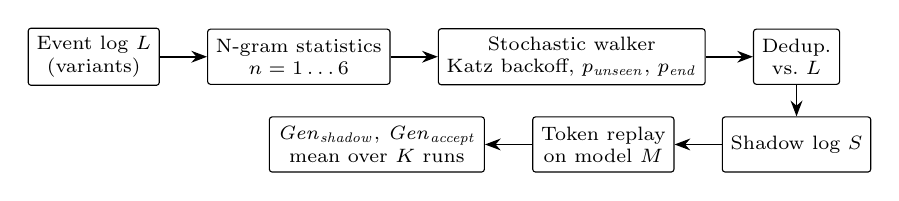
\begin{tikzpicture}[
  node distance=4mm and 6mm,
  box/.style={draw, rounded corners=1pt, align=center, font=\scriptsize, inner sep=3pt, minimum height=7mm},
  arr/.style={-{Stealth[length=2mm]}, semithick}
]
\node[box] (log) {Event log $L$\\(variants)};
\node[box, right=of log] (stats) {N-gram statistics\\$n = 1 \dots 6$};
\node[box, right=of stats] (walk) {Stochastic walker\\Katz backoff, $\punseen$, $\pend$};
\node[box, right=of walk] (dedup) {Dedup.\\vs.\ $L$};
\node[box, below=of dedup] (shadow) {Shadow log $S$};
\node[box, left=of shadow] (replay) {Token replay\\on model $M$};
\node[box, left=of replay] (score) {\genshadow, \genaccept\\mean over $K$ runs};
\draw[arr] (log) -- (stats);
\draw[arr] (stats) -- (walk);
\draw[arr] (walk) -- (dedup);
\draw[arr] (dedup) -- (shadow);
\draw[arr] (shadow) -- (replay);
\draw[arr] (replay) -- (score);
\end{tikzpicture}
\caption{ShadowGen pipeline. The generator is derived from the log only; the model under evaluation enters only at the replay step.}
\label{fig:pipeline}
\end{figure}

\subsection{Shadow log generation}
\label{sec:method:gen}

\subsubsection{Variant statistics.}
The log is compressed to its variants with case counts; every count below is weighted by how often the variant occurs ($\#v$). For each order $n\in\{1,\dots,N\}$ (default $N{=}6$) and each observed context $s$ (a length-$n$ activity sequence), we record the successor multiset $C_n(s)$, where $C_n(s)[a]$ is the frequency with which activity $a$ follows $s$, and separately the termination counts: $T_n(s)$, the number of occurrences of $s$, and $E_n(s)$, the number of those occurrences at the end of a trace.

\subsubsection{Katz backoff.}
At generation time the walker holds a partial trace $\sigma$ and resolves its decision context to the deepest order with adequate support. Let $\tau$ be a support threshold (default $5$). The \emph{resolved order} is the largest $n\le N$ such that the suffix $s=\mathrm{suffix}_n(\sigma)$ satisfies $|C_n(s)|_1 := \sum_a C_n(s)[a] \ge \tau$ \emph{and} the Good--Turing mass below is $<1$; otherwise $n$ is reduced, falling back ultimately to $n{=}1$. Thus $N$ is an upper bound, not a fixed operating point: on sparse logs the effective order is reduced naturally.

\subsubsection{Good--Turing novelty.}
For the resolved context $s$, the probability that the next activity is one never observed after $s$ is estimated as
\begin{equation}
\punseen(s) \;=\; \frac{N_1(s)}{\,|C(s)|_1\,}, \qquad N_1(s) = |\{a : C(s)[a]=1\}|,
\label{eq:gt}
\end{equation}
i.e., the number of singleton successors over the total successor count. With probability $\punseen(s)$ the walker \emph{mutates}; otherwise it \emph{exploits}.

\subsubsection{Mutation proposal (Katz-consistent).}
When a mutation fires, the inserted activity must be novel in the resolved context yet plausible. We draw it from the deepest \emph{shorter} context that offers a successor unseen at the resolved order. Let $R$ be the resolved order and $\mathit{seen}=\{a:C_R(s)[a]>0\}$. We scan $m=\min(|\sigma|,N),\dots,1$ and take the first $m$ for which $\{a:C_m(\mathrm{suffix}_m(\sigma))[a]>0\}\setminus\mathit{seen}\neq\emptyset$, sampling from that residual set; if none exists we fall back to global activity frequencies restricted to $\mathcal{A}\setminus\mathit{seen}$. A short observation fixes the search direction: a longer context's successor set is always contained in its suffix's, since every occurrence of $s$ is also an occurrence of its suffix $s'$ with the same next activity. Contexts of order $\ge R$ therefore add nothing new (orders $>R$ are subsets of the resolved successors, and order $R$ equals $\mathit{seen}$), so the proposal always finds its candidates at order $R{-}1$ or shorter, one level below the resolved order. \chg{An earlier design drew the mutated activity uniformly from $\mathcal{A}$ and thus injected behavior that was often process-impossible at that position; the Katz-consistent proposal replaces it.}

\subsubsection{Exploitation: two sampling modes.}
For a non-mutation step the walker samples a seen successor $a$ with weight $w(C(s)[a])$, normalized over the successor set. We support two weighting modes:
\begin{equation}
w_{\mathrm{mle}}(c)=c \qquad\text{vs.}\qquad w_{\mathrm{log}}(c)=\ln(c+1).
\end{equation}
The \texttt{mle} mode samples from the maximum-likelihood estimate of the next-activity distribution (proportional to observed frequency), so the shadow log mirrors the \emph{expected} future. The \texttt{log} mode deliberately flattens the distribution, up-weighting rare paths; it is a rare-behavior \emph{stress test}. \chg{The \texttt{mle} mode is the default and is what the evaluation reports; the calibration case for it is measured in Sect.~\ref{sec:eval:scale}.} The same weighting governs the mutation-proposal sampling, but never the mutation \emph{rate} of Eq.~\eqref{eq:gt}, which always uses raw counts.

\subsubsection{Context-aware termination.}
Whether the walk ends after context $s$ is decided by a termination probability resolved with the same backoff:
\begin{equation}
\pend(s) \;=\; \frac{E(s)}{T(s)}.
\end{equation}
Conditioning termination on the $n$-gram context (rather than the last activity alone) fixes premature termination when activities that legitimately end traces appear early in a generated trace.

\subsubsection{Deduplication and scoring.}
Each generated trace is compared against the set of original variants and regenerated if it is a copy (up to a retry cap), so the shadow log contains only unseen sequences. A shadow log $S$ of $\min(1000,|L|)$ traces is replayed on the model; generation and replay are repeated $K{=}5$ times (all randomness seeded). We report two scores: \genshadow{} (mean graded trace fitness, the headline) and \genaccept{} (fraction of perfectly replayed traces, the strict reading). We also report each score separately for shadow traces that contain a mutation and those that do not, which shows how a model handles genuinely novel events versus mere recombinations.

\subsection{Algorithm}
\label{sec:method:algo}
Algorithm~\ref{alg:gen} gives the generation procedure; statistics gathering and scoring are described above.

\begin{algorithm}[t]
\caption{Shadow-log generation (one iteration)}
\label{alg:gen}
\begin{algorithmic}[1]
\Require log $L$, order $N$, threshold $\tau$, count $T$, cap $M$, weighting $w$
\State build $C_n,T_n,E_n$ for $n=1..N$ from variants of $L$; collect starts, alphabet, variant set $\mathcal{V}$
\State $S\gets\emptyset$
\For{$i=1$ to $T$}
  \Repeat
    \State $\sigma\gets\langle\,$sample start activity$\,\rangle$; $\mathit{mut}\gets$ false
    \While{$|\sigma|<M$}
      \State resolve context $s$ by Katz backoff ($\tau$); compute $\punseen(s),\pend(s)$
      \If{$\mathit{rand}()<\pend(s)$} \textbf{break} \EndIf
      \If{$\mathit{rand}()<\punseen(s)$ \textbf{and} a novel candidate exists}
        \State append a Katz-consistent novel activity (weight $w$); $\mathit{mut}\gets$ true
      \Else
        \State append a seen successor sampled $\propto w(\cdot)$; \textbf{break} if dead end
      \EndIf
    \EndWhile
  \Until{$\sigma\notin\mathcal{V}$ \textbf{or} retry cap reached}
  \State $S\gets S\cup\{(\sigma,\mathit{mut})\}$
\EndFor
\State \Return $S$
\end{algorithmic}
\end{algorithm}

\subsection{Running example}
\label{sec:method:example}
Figure~\ref{fig:mutation} traces one mutation on a synthetic Sepsis pathway (seed $42$). Backoff does two jobs. It leaves the over-sparse order-6 context (seen five times, every successor once, so $\punseen=1$) for order~5 to set \emph{how often} to invent an event ($\punseen=1/35\approx3\%$); when the draw fires, it keeps backing off to order~4 to choose \emph{what} to invent (\textsf{Release-D}). The inserted activity is novel in the exact context, yet attested in a related shorter one, and the resulting trace (absent from the log) is flagged as a mutated shadow trace.

\begin{figure}[t]
\centering
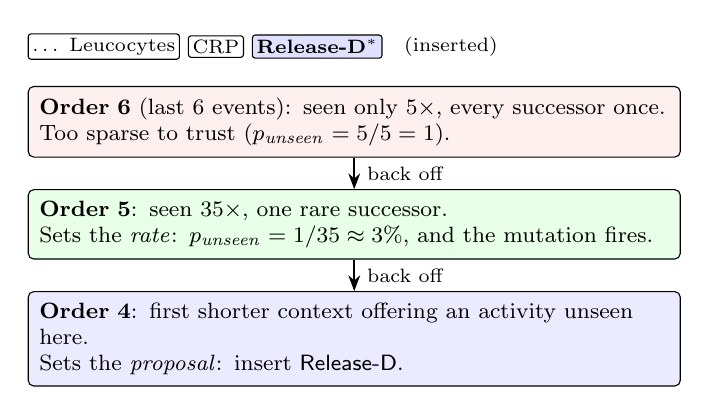
\begin{tikzpicture}[
  font=\footnotesize, node distance=4mm,
  lvl/.style={draw, rounded corners=2pt, align=left, inner sep=4pt, text width=80mm},
  ev/.style={draw, rounded corners=1pt, font=\scriptsize, inner sep=1.5pt},
  arr/.style={-{Stealth[length=2mm]}, semithick}
]
\node[ev] (a) {\dots\ Leucocytes};
\node[ev, right=1mm of a] (b) {CRP};
\node[ev, right=1mm of b, fill=blue!12] (c) {\textbf{Release-D}$^{*}$};
\node[right=1.5mm of c, font=\scriptsize] {(inserted)};
\node[lvl, fill=red!6, below=5mm of a.west, anchor=north west] (n6)
  {\textbf{Order 6} (last 6 events): seen only $5\times$, every successor once.\\
   Too sparse to trust ($\punseen=5/5=1$).};
\node[lvl, fill=green!9, below=of n6] (n5)
  {\textbf{Order 5}: seen $35\times$, one rare successor.\\
   Sets the \emph{rate}: $\punseen=1/35\approx3\%$, and the mutation fires.};
\node[lvl, fill=blue!8, below=of n5] (n4)
  {\textbf{Order 4}: first shorter context offering an activity unseen here.\\
   Sets the \emph{proposal}: insert \textsf{Release-D}.};
\draw[arr] (n6) -- node[right=1pt,font=\scriptsize]{back off} (n5);
\draw[arr] (n5) -- node[right=1pt,font=\scriptsize]{back off} (n4);
\end{tikzpicture}
\caption{Katz-consistent mutation (Sect.~\ref{sec:method:example}). Backoff sets both \emph{how often} to invent an event (the rate, resolved at order~5) and \emph{what} to invent (the proposal, found at order~4): novel in the exact context, yet attested in a related shorter one.}
\label{fig:mutation}
\end{figure}

\subsection{Time and space complexity}
\label{sec:method:complexity}
Let $|V|$ be the number of variants, $E_V=\sum_{v\in V(L)}|v|$ the total length of distinct variants, $A=|\mathcal{A}|$, $N$ the maximal order, $T$ the shadow-log size, $M\!\approx\!2\ell_{\max}$ the walk cap ($\ell_{\max}$ the longest variant), $K$ the iteration count, and $|M_P|$ the Petri-net size. Building the N-gram statistics is $O(N\,E_V)$ in time and $O(N\,D)$ in space for the $D$ stored $n$-grams; generation is $O(T\,M\,\bar b)$ with mean branching factor $\bar b\le A$, since context resolution and termination are memoized on the last-$N$ activities so each context is resolved once; token replay is $O(T\,M\,|M_P|)$. Per evaluated model the total is $O\!\big(K\,(N\,E_V + T\,M\,\bar b + T\,M\,|M_P|)\big)$.

Two observations matter. The cost is linear in the log \emph{through its variants}, not its cases: variant compression makes the metric scale with behavioral diversity rather than volume. This contrasts sharply with the leave-one-variant-out ground truth, which performs $|V|$ full discoveries ($O(|V|\cdot\mathrm{discover})$) and is orders of magnitude more expensive on variant-rich logs. The statistics are rebuilt once per iteration, contributing the factor $K$; this is an implementation artifact (Sect.~\ref{sec:impl:deviations}), not an intrinsic cost.

\subsection{Assumptions, scope, and limitations of the approach}
\label{sec:method:scope}
The method assumes a control-flow view (activity sequences; data, resources, and time are ignored) and a finite activity alphabet. It assumes the log is a representative-enough sample that local N-gram statistics are meaningful; on extremely sparse logs the backoff collapses toward $n{=}1$, reducing the metric to a 1-gram directly-follows generator, which remains a reasonable if weaker baseline \chg{(measured as the ablation in Sect.~\ref{sec:eval:scale})}. The shadow log models future behavior as recombinations of observed local patterns plus a calibrated tail of novel events; behavior driven by long-range or data-dependent dependencies beyond order $N$ is not captured. The metric exposes parameters ($N{=}6$, $\tau{=}5$, $K{=}5$), but they are fixed defaults: $N$ and $\tau$ are calibrated once (Sect.~\ref{sec:eval:setup}) and never tuned per dataset, and Katz backoff makes $N$ an upper bound that adapts downward on sparse logs. In use the metric is therefore as parameter-free as fitness and precision are. Finally, it measures only the generalization construct of Sect.~\ref{sec:method:construct} and is meant to be read alongside a precision metric, not in isolation.

% =====================================================================
\section{Implementation}
\label{sec:impl}

\subsection{Architecture}
\label{sec:impl:arch}
The metric is implemented in Python on top of PM4Py~\cite{berti2019pm4py}. \chg{The code is an algorithm registry of frozen modules: each design stage is preserved as the exact code that produced its numbers, so every result is regenerable and the 1-gram ablation (Sect.~\ref{sec:eval:scale}) is an earlier module loaded by name.} The benchmark layer adds model preparation, per-method bridges (including subprocess bridges to Java/Docker baselines), the ground-truth scripts, and \chg{a runner with a uniform \texttt{evaluate\_miner(log, miner)} entry point}.

\subsection{Key design decisions}
\label{sec:impl:decisions}
\textbf{Variant compression.} Statistics and deduplication operate on variants weighted by case count, making preprocessing independent of case volume (Sect.~\ref{sec:method:complexity}). \textbf{Determinism.} All random number generators are seeded ($\mathit{seed}{=}42$) so that every cell is reproducible\chg{; the residual nondeterminism of the replay library itself is measured in Sect.~\ref{sec:eval:threats}}. \textbf{Provenance.} Every (dataset, miner, method) cell writes a sidecar JSON with exact parameters, raw per-iteration scores, runtime, and integrity counters (\texttt{duplicates\_kept} and \texttt{truncated\_traces}, which surface any deviation of the shadow log from its specification); these files are the single source of truth for all tables, and a result without a matching config is invalid.

\subsection{Baseline integration realities}
\label{sec:impl:baselines}
Integrating the eight external baselines surfaced engineering realities that materially affect the evaluation and must be reported as such. The PM4Py metric (M2) is a one-line library call. AVATAR (M5) runs in a TensorFlow~1 Docker image and required a greedy longest-match decoder to reconstruct multi-word activity names from the GAN's token output. SpeciAL (M7) is a Python package used directly\chg{; on D5 we use the released PyPI package (\texttt{special4pm} 0.1.3), on D1--D4 the source copy provided by the authors' repository, a version skew we disclose (Sect.~\ref{sec:eval:threats})}. \chg{Anti-alignments (M4) and pattern-based generalization (M8) run only on the small logs and finish only part of the miners} (Sect.~\ref{sec:eval:feasibility}). A third, entropic relevance (M3), needs a Petri-net-to-stochastic-automaton conversion, reported two ways. \chg{At scale we approximate it with a per-miner DFG simulation (PM4Py \texttt{play\_out}, 5\,000 traces) converted to a probability automaton via the open-source \texttt{relevance.jar} from the Entropia toolset~\cite{polyvyanyy2020entropia} (JDFG2Aut + Relevance); this runs on all five datasets but takes its transition probabilities from the simulated DFG frequencies, not from the net. For the construct test we build the automaton properly, from each net's reachability graph with silent transitions collapsed and the result determinized over visible labels, probabilities from log replay, scored with Entropia's entropic relevance directly. The proper conversion is exact but bounded: on D1 two of the six real miners have no finite automaton (unbounded or state-exploding reachability), and where it runs it fails the flower litmus (Sect.~\ref{sec:eval:feasibility}). The relevance computation and the proper conversion are additionally reimplemented in plain Python and validated against the Entropia tool ($3$-decimal agreement on every D1 automaton; \texttt{benchmark/m3\_entropic\_relevance.py}), so the construct test does not depend on the external Java toolchain.}

Bootstrap (M6adapted) is a construct-faithful adaptation: its target, model--system recall~\cite{polyvyanyy2022bootstrap}, is exactly the construct we adopt (Sect.~\ref{sec:related}). Our bridge runs the genuine \texttt{bsgen} bootstrap-with-breeding \emph{sampler} and scores the bred traces by PM4Py token-replay fitness, i.e.\ a \emph{graded} model--system recall, the way \genshadow{} grades the shadow log. \chg{The sampler itself is our reimplementation of the paper's published algorithms (the original source is not public); it reproduces the published D1 values within $0.008$ on every cell.} We deliberately avoid the Entropia \texttt{-bgen} tool's harmonic mean of model--system precision and recall: that F-measure folds precision back in and is no longer the paper's recall-based generalization. It scores the flower model $0.18$ instead of $1.0$ on D1, failing the litmus of Sect.~\ref{sec:method:construct}\chg{, and we carry it through the benchmark as its own method id (\texttt{M6original}) so the contamination stays measurable at scale (Sect.~\ref{sec:eval:scale})}. The price of our choice is twofold. First, M6adapted as we report it is not the off-the-shelf Entropia \texttt{-bgen} output but our own token-replay scoring of its genuine \texttt{bsgen} sampler, so it is an adaptation, not a drop-in published baseline. Second, that scoring is the conformance core of our metric and of R1, a shared-ruler effect we flag in Sect.~\ref{sec:eval:threats}.

\subsection{Deviations from the formal method}
\label{sec:impl:deviations}
Three deviations are worth recording. (i) As noted in Sect.~\ref{sec:method:complexity}, the N-gram model is rebuilt each of the $K$ iterations rather than once; this is a performance artifact, not a semantic one. (ii) The strict reading counts a shadow trace as accepted when PM4Py's token replay flags it as perfectly fitting (\texttt{trace\_is\_fit}). That flag is a fast but approximate test of language membership, which is properly decided by a cost-zero alignment. On nets with invisible (silent) or duplicate-label transitions the two can disagree, so our acceptance number is a proxy\chg{; Sect.~\ref{sec:eval:accept} quantifies the disagreement per net class}. (iii) \chg{The data-driven length cap never binds on D1/D2 (\texttt{truncated\_traces}${=}0$). On the deep-trace logs it does, and it pays: on D4 the cap alone improves calibration from MAE $0.038$ to $0.027$ (log weighting throughout, cap the only change; the headline MLE configuration reaches $0.016$).}

% =====================================================================
\section{Evaluation}
\label{sec:eval}
This is an algorithmic, quantitative contribution, so we evaluate experimentally. We measure how well each metric agrees with an empirical generalization ground truth across discovery configurations and datasets, and we attribute the proposed metric's behavior to specific design decisions through \chg{a measured ablation}.

\subsection{Experimental setup}
\label{sec:eval:setup}

\subsubsection{Datasets.}
From a profiled catalog of \chg{$21$} public logs we selected five (Table~\ref{tab:datasets}) spanning trace depth, variant diversity, scale, and, most deliberately, \chg{trace-based log representativeness (TLRA, ranging $0.19$--$0.95$), the axis shown to impact the accuracy of generalization estimation~\cite{karunaratne2024representativeness}}. The same evaluation battery runs on every dataset. We present D1 (Sepsis) in full as the primary case, carrying the cross-paradigm comparison and its figures; D2 (BPI 2013 Incidents) corroborates the litmus and the acceptance reading\chg{; D3--D5 extend the study to logs of up to $2.5$ million events (Sect.~\ref{sec:eval:scale})}.

\begin{table}[t]
\centering
\caption{Benchmark datasets. TLRA $=1-|V|/|L|$.}
\label{tab:datasets}
\setlength{\tabcolsep}{3pt}
\footnotesize
\begin{tabular}{@{}llrrrrr@{}}
\toprule
ID & Log & Cases & Events & Variants & Avg.\ len & TLRA \\
\midrule
D1 & Sepsis~\cite{mannhardt2016sepsis} & 1{,}050 & 15{,}214 & 846 & 14.5 & 0.19 \\
D2 & BPI 2013 Incidents\chg{~\cite{steeman2013bpi}} & 7{,}554 & 65{,}533 & 1{,}511 & 8.7 & 0.80 \\
D3 & BPI 2017\chg{~\cite{vandongen2017bpi}} & 31{,}509 & 1{,}202{,}267 & 15{,}930 & 38.2 & 0.49 \\
D4 & BPI 2018\chg{~\cite{vandongen2018bpi}} & 43{,}809 & 2{,}514{,}266 & 28{,}457 & 57.4 & 0.35 \\
D5 & BPI 2019\chg{~\cite{vandongen2019bpi}} & 251{,}734 & 1{,}595{,}923 & 11{,}973 & 6.3 & 0.95 \\
\bottomrule
\end{tabular}
\end{table}

\subsubsection{Discovery configurations.}
Eight miners span the construct's poles: a filtered trace model (top-50 variants by frequency; the full trace model is intractable to replay on variant-rich logs), Alpha and Alpha+~\cite{vanderaalst2004alpha}, Heuristics default and strict~\cite{weijters2006hm}, Inductive strict and infrequent~\cite{leemans2013im,leemans2014imf}, and a flower model. Models are discovered once per (dataset, miner) cell and shared by all methods.

\subsubsection{Methods and ground truth.}
\chg{Our metric is M1: ShadowGen as specified in Sect.~\ref{sec:method} (release id v2.6-mle; benchmark id M1g). A single ablation baseline (benchmark id M1a) replaces the variable-order model by its 1-gram floor, a directly-follows generator with the same Good--Turing novelty and termination machinery, and isolates what deep context contributes (Sect.~\ref{sec:eval:scale}).} External baselines are M2--M9 (Sect.~\ref{sec:related}). Reference metrics are R1 (variant-based 5-fold CV fitness, 3 shuffles), R2 (leave-one-variant-out), and R3 (replay of uniformly random traces, a floor). An acceptance-based variant, R1-accept, measures the fraction of held-out traces replayed perfectly and validates the acceptance reading.

\subsubsection{Protocol and agreement criteria.}
Each cell is evaluated with its method's stochasticity protocol (our metric: $5$ iterations of $1{,}000$ shadow traces, mean $\pm$ std; seed $42$). Agreement with the ground truth is reported on \emph{four criteria}: Pearson (calibration shape), Spearman and Kendall's $\tau_b$ (ordering), mean absolute error (MAE, absolute calibration), and discriminative spread (max$-$min over the six non-degenerate miners). All four are computed over those six miners; the two poles are excluded and reported separately as litmus values. Rank correlation alone is too weak a test: as Sect.~\ref{sec:eval:external} shows, a random-replay baseline also reaches Spearman and Kendall $1.0$. The context order was fixed at $N{=}6$ via a mutation-rate sweep on BPI 2017 (the realized mutation rate peaks at $N{=}6$ and declines beyond, as backoff increasingly rejects sparse contexts; Fig.~\ref{fig:nsweep}), and $N{=}6$ is held fixed across all datasets so the metric is never tuned per dataset.

\chg{\emph{Compute budget.} Every method is granted $1$ hour of metric time per (dataset, miner) cell. Model discovery is excluded: models are discovered once per cell, cached, and shared by all methods. The references (R1, R2, R1-accept) are exempt; they define the ground truth. A cell that does not return within the budget is recorded as a sentinel with the measured evidence, excluded from the agreement statistics, and not re-run. Since the working metrics complete a cell in seconds, this turns runtime into a first-class outcome: a method's inability to finish is a result, not an omission.}

\begin{figure}[t]
\centering
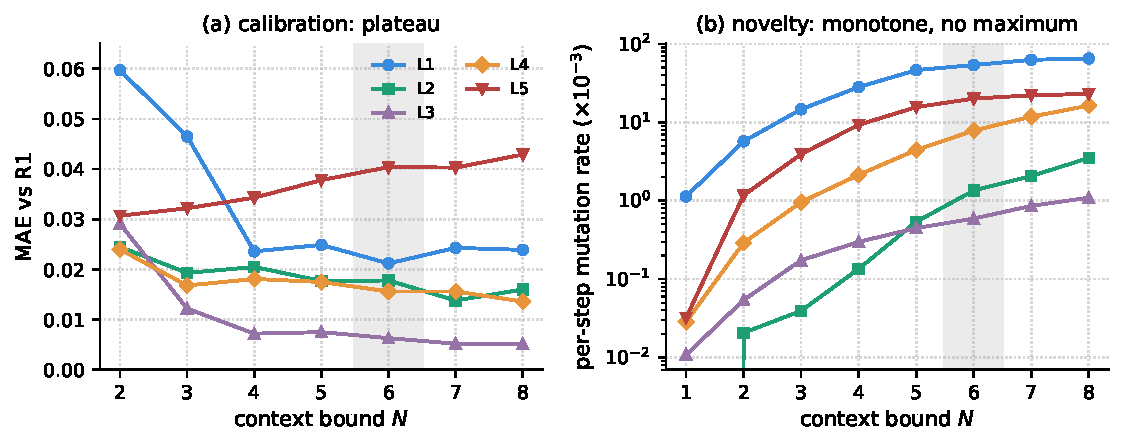
\includegraphics[width=0.62\textwidth]{figures/fig_nsweep.pdf}
\caption{Realized mutation rate vs.\ N-gram order on BPI 2017 (the one calibration of the metric). The rate climbs to a peak at $N{=}6$ and declines beyond, as Katz backoff increasingly rejects over-sparse high-order contexts; $N{=}6$ is then held fixed on every dataset.}
\label{fig:nsweep}
\end{figure}

\subsection{Feasibility results}
\label{sec:eval:feasibility}
\chg{Under the compute budget, two published metrics (M4, M8) return on too few models to be scored: each finishes at most two of the six real miners on any log, on the small logs only, and neither returns a real miner at scale. Anti-alignments (M4) run the published implementation~\cite{vandongen2016anti} under the same budget. It scores three of the eight D1 models and three of the eight D2 models, never more than two of the six real miners, nothing on D3 or D4, and only the trace pole on D5; on D4 the $2.5$ million event log does not finish even the alignment step within the hour. On D1 Inductive-infrequent aborts inside the solver on an internal index overflow, Alpha+ reaches $1\%$ of its traces within the hour, \chg{Heuristics reaches $87\%$ at the kill (the one near-miss) and Inductive-strict $0.1\%$,} and the flower model never returns. Where M4 does score, the trace model reads $0.0$, the correct pole. Pattern-based generalization (M8)~\cite{reissner2022pattern} fails similarly: it scores three of the eight D2 models in seconds (Heuristics $0.99$, Heuristics-strict $0.999$, and the trace model), crashes with a null alignment on the other five, and returns nothing on D1, D3, D4, or D5. \chg{Unlike M4, it exposes no progress counter, so its non-returns are wall-clock kills without a measured progress percentage.} Its $0.90$ on the trace model is the wrong pole, a memorizing model read as general. Neither returns all six real miners on any log, so neither can be placed on the four-criteria agreement. Against seconds per cell for the working metrics, neither finishes every model on even the smallest real log, and both fail outright at scale.} \chg{Entropic relevance (M3) is feasible on all five logs as a directly-follows approximation (Sect.~\ref{sec:impl:baselines}), but its agreement with the ground truth is unstable (per-log Pearson against R1 from $-0.80$ to $+0.95$), so we do not read it as tracking held-out fitness. Computed properly, from a stochastic automaton built from each net's reachability graph, it confirms the problem directly: on D1 two of the six real miners (Alpha, Heuristics) have no finite automaton, and on the four that convert it places the flower model mid-field ($52$ bits against $22$ to $62$ for the real models), failing the flower litmus of Sect.~\ref{sec:method:construct}. Extended to all five logs, the proper conversion builds on $24$ of $40$ cells (all $8$ on the $4$-activity D2, $3$ of $8$ on D5, at a $150$k-marking cap); the deeper the concurrency, the fewer nets convert. Entropic relevance scores a fitness and precision blend, not generalization, so we keep it out of the agreement tables.}

\chg{Negative-event generalization (M9)~\cite{vandenbroucke2014negative}, run through the CoBeFra implementation in its shipped configuration (weighted artificial negatives with token replay), does not track held-out generalization on any log. On D1 it is anti-correlated with the ground truth over the six real miners (Pearson $-0.55$, more negative than PM4Py), rating the well-generalizing Heuristics models near zero; on the four-activity D2 and the short-trace D5 it collapses, scoring every model $1.0$ including the memorizing trace pole, so it discriminates nothing (MAE $0.18$ and $0.23$). It passes the flower litmus on the small logs ($1.0$) but mis-anchors the trace pole ($0.48$ on D1, $1.0$ on D2 and D5), and it does not scale: on D3 only two of the six real miners return within the hour and on D4 (mean trace length $57$) none do. Its scores are also non-deterministic on nets with silent transitions (D1 Inductive-infrequent, std $0.07$ across runs), the same token-replay tie-breaking that affects the acceptance proxy (Sect.~\ref{sec:eval:accept}). Because it is degenerate on D2 and D5 and infeasible at scale on D3 and D4, no scorable four-criteria result exists; like structural counting and entropic relevance it measures a fitness and precision blend rather than generalization, so we keep it out of the agreement tables. The run and driver are in \texttt{benchmark/m9/}.}

\chg{AVATAR (M5) meets the one-hour budget on no log and is therefore a budget sentinel on all five; its two small-log scorecards, obtained off-protocol (two of the $3$--$5$ published runs), are read for the flower litmus and the off-protocol calibration illustration (Figs.~\ref{fig:calibration},~\ref{fig:pareto}; Sect.~\ref{sec:eval:external}), never as agreement rows. The evidence is measured: a reduced D1 anchor ($3$ of $100$ pre-epochs, $100$ of $5{,}000$ adversarial steps) already needs $88$ minutes on the smallest log, its per-step rate ($45$\,s) projects the full published configuration to ${\sim}3$--$4$ days of wall time (over $400$ CPU-hours) per log on benchmark-class CPU hardware, D3 spent its full hour without leaving GAN pretraining, and D4 was killed at both a $16$ and a $24$\,GB memory cap. The authors themselves report hours of GPU training per log~\cite{theis2020avatar}, so on either hardware class AVATAR sits orders of magnitude beyond the one-hour budget. Its published configuration also caps sequences at $20$ events, below the mean trace length of D3 ($38.2$) and D4 ($57.4$), so its scores there would truncate the behavior generalization asks about; raising the cap is a configuration change that only adds to the already prohibitive cost.}

\chg{Two boundary results at scale: the published Entropia \texttt{-bgen} tool needs $6$ to $10$ minutes per D4 cell (five of eight cells return within the hour; the other three fail inside the tool), and SpeciAL scores six of eight D5 cells (Alpha and Alpha+ exceed the hour). In sum, M2, M3, M6adapted, M6original, and M7 score at scale with these sentinels; M5 exceeds the budget on every log; M4 and M8 return only on the small logs, always leaving models unscored, and no real miner at scale. We also disclose five D4 cells kept in the tables despite overrunning the hour before returning, against the sentinel rule: M2 Inductive-strict ($3.5$\,h), the 1-gram ablation's Inductive-strict ($4.0$\,h), SpeciAL Heuristics-strict ($2.2$\,h) and Heuristics ($1.2$\,h), and the R3 floor's Inductive-strict ($1.2$\,h). They are real measurements, and sentineling them would only remove scored cells from baselines that already fail, so we keep and flag them.}

\subsection{Cross-paradigm comparison on D1}
\label{sec:eval:external}

% tab:external moved to the appendix (Sect.~\ref{sec:appendix:external}, Raw cross-paradigm scores on D1)

\begin{table}[t]
\centering
\caption{Agreement with R1 on D1 (six real miners) and the flower litmus. $\tau_b$ is Kendall's tau-b. \chg{$^{*}$M6adapted uses adapted scoring (Sect.~\ref{sec:impl:baselines}).}}
\label{tab:corr}
\setlength{\tabcolsep}{4.5pt}
\footnotesize
\begin{tabular}{@{}lrrrrrr@{}}
\toprule
Method & Pearson & Spearman & $\tau_b$ & MAE & Spread & Flower \\
\midrule
\chg{ShadowGen (ours)}  & 0.996 & 1.00 & 1.00 & 0.023 & 0.71 & 1.00 \\
M2 PM4Py         & $-$0.35 & $-$0.43 & $-$0.20 & 0.17 & 0.09 & 0.91 \\
M6adapted$^{*}$ & 0.998 & 1.00 & 1.00 & 0.018 & 0.74 & 1.00 \\
M7 SpeciAL       & 0.12 & $-$0.46 & $-$0.41 & 0.21 & 0.26 & 0.80 \\
R3 Random        & 0.83 & 1.00 & 1.00 & 0.28 & 0.49 & 1.00 \\
\bottomrule
\end{tabular}
\end{table}

Table~\ref{tab:corr} compares the paradigms against the cross-validation ground truth. Four findings stand out.
\begin{enumerate}
  \item Generative and resampling paradigms track held-out fitness; structural and diversity paradigms do not. The most widely available metric (M2) correlates negatively with the ground truth, compresses six structurally very different models into a spread of \chg{$0.09$}, and \chg{ranks the two Alpha variants, the ground truth's bottom pair, above every other model}. This is direct evidence that visit-frequency counting does not measure held-out generalization.
  \item Rank correlation alone is a low bar. The random-replay floor R3 attains Spearman and $\tau_b$ of $1.0$, because the Sepsis miners differ so strongly in permissiveness that almost any test orders them correctly. Validation must rest on the full set of criteria, which is where \chg{ShadowGen} and bootstrap (MAE $0.023$/\chg{$0.018$}, spreads $0.71$/$0.74$) separate from R3 (MAE $0.28$, spread $0.49$).
  \item The flower litmus sorts the field. Pure-acceptance metrics (\chg{ShadowGen}, M6adapted, R1--R3) score the flower model $1.0$, as the construct requires; M2, M7, and \chg{especially AVATAR (off-protocol flower $0.40$; Sect.~\ref{sec:eval:feasibility})} reveal precision/structure contamination. That M6adapted lands in the first group is independent corroboration, not coincidence: the bootstrap metric is itself defined as model--system recall~\cite{polyvyanyy2022bootstrap}, so a separate, published generalization measure also rates the flower model maximally general. \chg{AVATAR's} low flower score, by contrast, follows from its construct (a harmonic mean of fitness and precision~\cite{theis2020avatar}, i.e.\ an F-measure), which also explains \chg{why it scatters off the calibration line (Fig.~\ref{fig:calibration})}.
  \item Bootstrap is the closest competitor, with a caveat. M6adapted matches our calibration, but it scores with token-replay fitness, the same conformance engine as R1 and our own metric; part of its tight agreement is a shared-ruler effect rather than independent corroboration (Sect.~\ref{sec:eval:threats}).
\end{enumerate}

The agreement is robust to the choice of cross-validation reference\chg{: against} the finer-grained leave-one-variant-out (R2\chg{, $50/846$ variants sampled}), ShadowGen's ranking is identical (Kendall $\tau_b{=}1.0$) and its calibration is unchanged on D1 (MAE $0.014$); on D2 the ranking again holds while calibration stays strong (Pearson $0.97$, MAE $0.048$). The verdicts on every baseline are the same under R1 and R2. \chg{The agreement is robust to the miner sample too: extending D1 to eleven discovery configurations (the six real miners plus five threshold variants) holds the calibration at Pearson $0.997$, with a bootstrap $95\%$ confidence interval of $[0.953, 0.999]$ (MAE $0.015$, interval $[0.010, 0.021]$), so it is not an artifact of a six-point sample.}

The litmus failures also replicate on D2: PM4Py scores the flower model $0.88$, AVATAR $0.74$ \chg{(off-protocol)}, and SpeciAL $0.94$, all below the $1.0$ the construct requires, while \chg{ShadowGen} and the references stay at $1.0$.
Figure~\ref{fig:calibration} plots each metric against the cross-validation ground truth directly on D1 \chg{(the D2 counterpart is qualitatively identical, Table~\ref{tab:scale} D2 column, and adds no method not already shown)}; the raw per-cell scores are tabulated in the appendix (Table~\ref{tab:external}).

\begin{figure}[t]
\centering
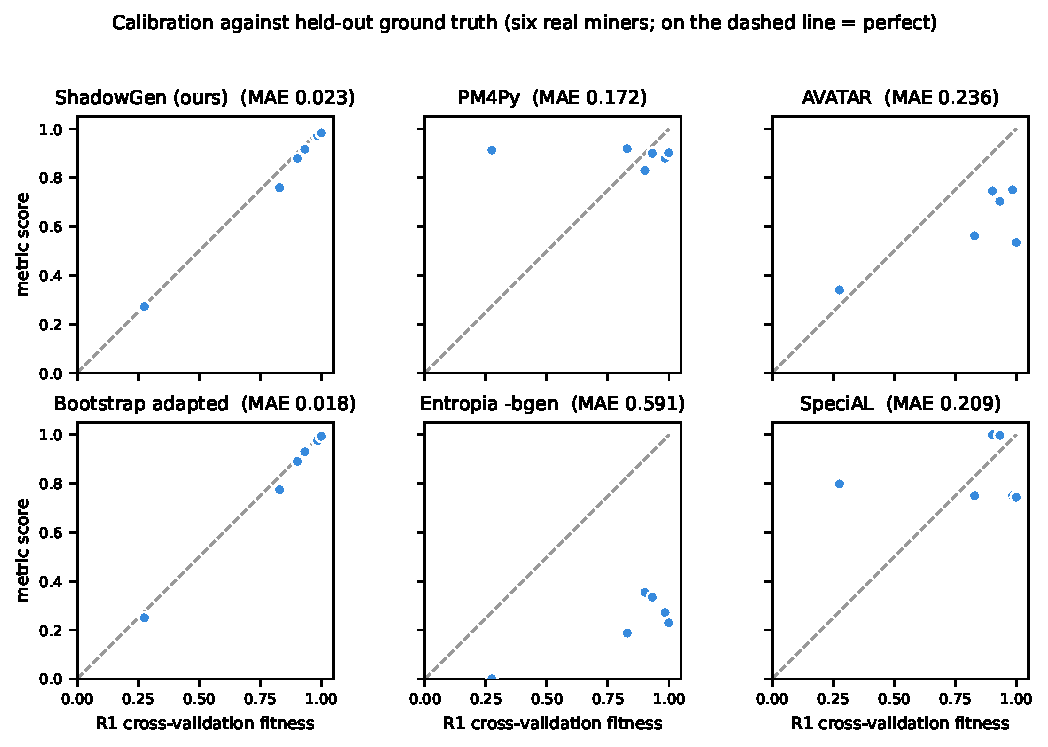
\includegraphics[width=\textwidth]{figures/fig_calibration_d1v2.pdf}
\caption{Per-method calibration against the cross-validation ground truth on D1 (six real miners; each point is one miner, dashed line $y{=}x$). The generative and resampling metrics (ShadowGen, Bootstrap adapted) sit on the line\chg{; the published Entropia \texttt{-bgen} F-measure of the same bootstrap sample sits far below it (its F1 folds precision in, Sect.~\ref{sec:eval:m6})}; PM4Py forms a flat high band that ignores the ground-truth gradient: it rates the pathological Alpha model (at R1$\approx0.27$) as $0.91$; \chg{AVATAR (shown off-protocol, Sect.~\ref{sec:eval:feasibility})} and SpeciAL scatter off the line. Reading the vertical axis alone, a metric that spreads its six miners discriminates between them, whereas PM4Py compresses them into a narrow band.}
\label{fig:calibration}
\end{figure}

\subsection{What contaminates a generalization score: a controlled bootstrap study}
\label{sec:eval:m6}
Bootstrap generalization is published as a generalization metric in its own right~\cite{polyvyanyy2022bootstrap}, so it is worth asking why the number a user typically reads off it (the Entropia \texttt{-bgen} F1 of model--system precision and recall) fails the flower litmus. Because one bred \texttt{bsgen} sample can be scored several ways, we hold the sampler fixed and vary only the scoring (Table~\ref{tab:m6}).

\begin{table}[t]
\centering
\caption{The same \texttt{bsgen} bootstrap sample on D1, scored four ways, vs R1 (six real miners). Only the readings free of precision pass the flower litmus.}
\label{tab:m6}
\setlength{\tabcolsep}{5pt}
\footnotesize
\begin{tabular}{@{}lrrrrl@{}}
\toprule
Reading of the bootstrap sample & Pearson & $\tau_b$ & MAE & Flower & litmus \\
\midrule
M6original \texttt{-bgen} F1(prec, rec) & 0.87 & 0.20 & 0.59 & 0.18 & fail \\
\quad its precision component & 0.82 & 0.20 & 0.68 & 0.10 & fail \\
\quad its \textbf{recall} component & 0.98 & 0.73 & 0.11 & 1.00 & pass \\
\textbf{M6adapted} (token-replay) & 1.00 & 1.00 & 0.018 & 1.00 & pass \\
\bottomrule
\end{tabular}
\end{table}

The two readings that include precision fail the litmus (flower $0.18$, $0.10$) and miscalibrate badly (MAE $0.59$, $0.68$); the two recall-only readings pass and track R1. The F1 still reaches Pearson $0.87$, yet its MAE $0.59$ and flower $0.18$ expose it, which is why the protocol uses four criteria and not one. So it is the precision component, not the bootstrap sampler, that throws the bootstrap off, and this is why we report it (M6adapted) by token-replay fitness, faithful to the paper's recall construct (Sect.~\ref{sec:impl:baselines}). \chg{This is the construct argument of Sect.~\ref{sec:method:construct} made empirical: folding precision into a generalization score is not merely conceptually wrong, it measurably destroys calibration and the litmus. Section~\ref{sec:eval:scale} shows the same split at scale: the adaptation stays calibrated on every log, the F1 reading fails everywhere.}

{\color{chgblue}
\subsection{Results at scale: D3--D5}
\label{sec:eval:scale}
The three large logs multiply the event volume by up to $165\times$ over D1 and change the regime: deeper traces (D4 averages $57.4$ events), larger variant spaces (up to $28{,}457$), and both extremes of representativeness (TLRA $0.35$--$0.95$). Table~\ref{tab:scale} reports the agreement with R1 on all five logs; Fig.~\ref{fig:calscale} plots our metric's 30 real-miner cells against the ground truth.

\begin{table}[t]
\centering
\caption{Agreement with R1 on all five logs (six real miners each): Pearson / MAE per log, and the flower-litmus range. \chg{AVATAR is a budget sentinel on all five logs (Sect.~\ref{sec:eval:feasibility});} the SpeciAL D5 entry covers the four miners that returned within budget; \chg{the Entropia \texttt{-bgen} D4 entry covers the three that returned;} M4/M8 return too few cells to rank.}
\label{tab:scale}
\setlength{\tabcolsep}{2.2pt}
\scriptsize
\begin{tabular}{@{}l cc cc cc cc cc c@{}}
\toprule
 & \multicolumn{2}{c}{D1} & \multicolumn{2}{c}{D2} & \multicolumn{2}{c}{D3} & \multicolumn{2}{c}{D4} & \multicolumn{2}{c}{D5} & Flower \\
\cmidrule(lr){2-3}\cmidrule(lr){4-5}\cmidrule(lr){6-7}\cmidrule(lr){8-9}\cmidrule(lr){10-11}
Method & Pear. & MAE & Pear. & MAE & Pear. & MAE & Pear. & MAE & Pear. & MAE & \\
\midrule
ShadowGen (ours) & .996 & .023 & .994 & .019 & .999 & .006 & .999 & .016 & .986 & .043 & 1.00 (all) \\
M6adapted & .998 & .018 & .978 & .034 & .999 & .006 & .993 & .020 & .998 & .014 & 1.00 (all) \\
M2 PM4Py & $-$.35 & .172 & .41 & .184 & $-$.65 & .135 & $-$.53 & .208 & $-$.33 & .229 & .88--.98 \\
M7 SpeciAL & .12 & .209 & .12 & .158 & .63 & .122 & .76 & .162 & $-$.24 & .079 & .76--.94 \\
M6original (\texttt{-bgen} F1) & .87 & .591 & .95 & .250 & .13 & .760 & .82 & .724 & .98 & .619 & .05--.53 \\
R3 Random floor & .83 & .281 & .97 & .116 & .70 & .265 & .88 & .176 & .84 & .196 & 1.00 (all) \\
\bottomrule
\end{tabular}
\end{table}

\begin{figure}[t]
\centering
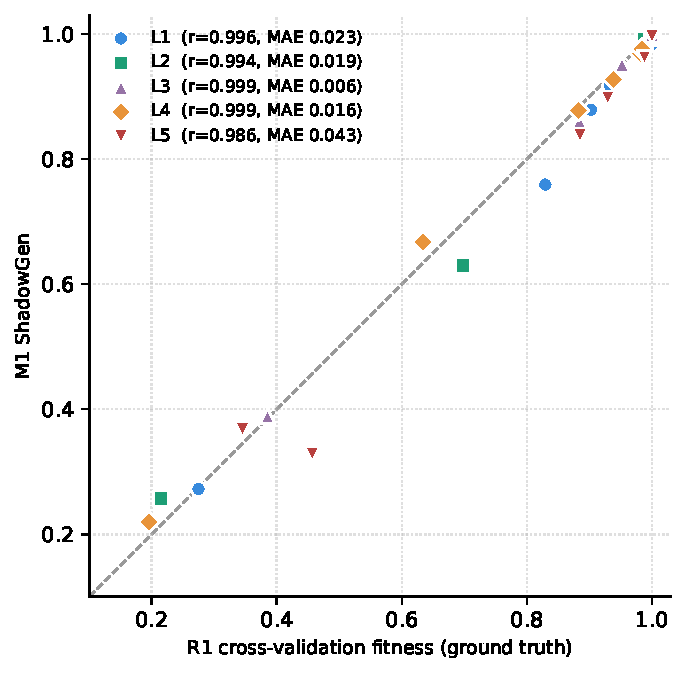
\includegraphics[width=0.7\textwidth]{figures/fig_calibration_scale.pdf}
\caption{ShadowGen against the R1 ground truth on the six real miners of every log (30 cells, dashed line $y{=}x$). The calibration measured on D1/D2 carries to logs of $2.5$ million events.}
\label{fig:calscale}
\end{figure}

Six findings.
\begin{enumerate}
  \item \emph{The calibration holds at scale.} ShadowGen tracks R1 on every log: Pearson $0.986$--$0.999$, MAE $0.006$--$0.043$, spread $0.61$--$0.76$, flower exactly $1.0$ everywhere. The ranking is perfect on D1, D2, and D4; on D3 and D5 exactly one adjacent pair swaps (Spearman $0.94$). Both swaps are benign: on D3 the pair is separated by $0.0004$ in R1 (a tie for practical purposes), on D5 it is the two Alpha variants, both scored far below the field by metric and ground truth alike.
  \item \emph{A second generator lands on the same calibration.} The bootstrap adaptation (M6adapted) co-leads on every log (MAE $0.006$--$0.034$, flower $1.0$). We read this as corroboration rather than competition: two independently designed synthetic-log generators (bootstrap resampling with crossover breeding; a variable-order N-gram model with calibrated novelty), scored by the same acceptance reading, agree with the ground truth and with each other. The generative paradigm, not one specific generator, carries the result. The practical difference is cost (median $36.9$\,s against our $14.9$\,s per model) and the principled novelty injection that resampling lacks (Sect.~\ref{sec:related}).
  \item \emph{The precision contamination of the published reading replicates everywhere.} The Entropia \texttt{-bgen} F1 of the same sampler fails the litmus on every log (flower $0.05$--$0.53$) and miscalibrates by an order of magnitude more than the recall-faithful adaptation (MAE $0.250$--$0.760$). The D1 diagnosis of Sect.~\ref{sec:eval:m6} is not a D1 artifact.
  \item \emph{PM4Py fails on every log.} Its Pearson is negative on D1, D3, D4, and D5 and $0.41$ on D2, its spread never exceeds $0.14$, and it fails the flower litmus on all five ($0.88$--$0.98$). SpeciAL shows no stable relationship either (Pearson $-0.24$ to $0.76$) and rates the memorizing trace model at $1.0$ on every log, the opposite pole error.
  \item \emph{Rank correlation stays a low bar at scale.} The random-replay floor R3 orders the miners nearly perfectly on every log (Spearman $0.94$--$1.0$, $\tau_b$ $0.87$--$1.0$) while miscalibrating by MAE $0.116$--$0.281$. The four-criteria protocol is what separates the calibrated metrics from the floor, on every dataset.
  \item \emph{Deep context earns its keep on deep logs.} The 1-gram ablation is competitive on the two short-trace, high-TLRA logs (D2 MAE $0.036$; on D5 it is even better calibrated, $0.026$ against $0.043$) but falls behind by an order of magnitude on D3 (MAE $0.066$ against $0.006$), by $2.3\times$ on D4, and by $3\times$ on D1. This confirms the prediction registered in the two-log study: the variable-order model pays off exactly where decisions depend on deep context, and the honest converse is that on shallow repetitive logs a directly-follows generator suffices. The weighting choice behaves the same way: the default MLE weighting calibrates better than the log-weighted stress mode on D1--D4 (MAE $0.023$/$0.019$/$0.006$/$0.016$ against $0.068$/$0.045$/$0.046$/$0.027$), while on D5, the same shallow and repetitive regime, the flattened mode is slightly better calibrated ($0.035$ against $0.043$). The generator premise test (Sect.~\ref{sec:eval:genval}) shows the same by an independent measure: on D3 only the full model produces exact matches of held-out real variants ($8.6\%$ vs $0\%$).
\end{enumerate}

One registered prediction is refuted. Following~\cite{karunaratne2024representativeness} we predicted that calibration error grows as TLRA falls. It does not: the lowest MAE occurs at TLRA $0.49$ (D3, $0.006$) and the highest at TLRA $0.95$ (D5, $0.043$), with no monotone trend across the five logs. At these scales, trace depth and alphabet size govern the difficulty of generalization estimation at least as much as trace-based representativeness does.
}

\subsection{The acceptance reading}
\label{sec:eval:accept}
\genaccept{} reports the fraction of shadow traces replayed perfectly, the strict membership-shaped reading. It is best read not as a competing quality score (it is bimodal and rank-uninformative, see below) but as a diagnostic that decomposes the graded one: $\genshadow$ is real acceptance plus partial credit, and the per-model gap between the two says how much of a score is real. Acceptance values must be validated against an acceptance-based ground truth (R1-accept: the fraction of held-out real traces replayed perfectly). \chg{Against the matching ground truth, \genaccept{} reaches Pearson $0.992$--$0.999$ and MAE $0.021$--$0.076$ on D1, D2, D3, and D5 (per log, Table~\ref{tab:accept-scale}), and the poles anchor on every log including D4 (flower model $1.00$ exactly, trace model at or below $0.003$), in metric and ground truth alike.} The D1 detail below carries the argument (Table~\ref{tab:accept}, Fig.~\ref{fig:accept}).

\begin{figure}[t]
\centering
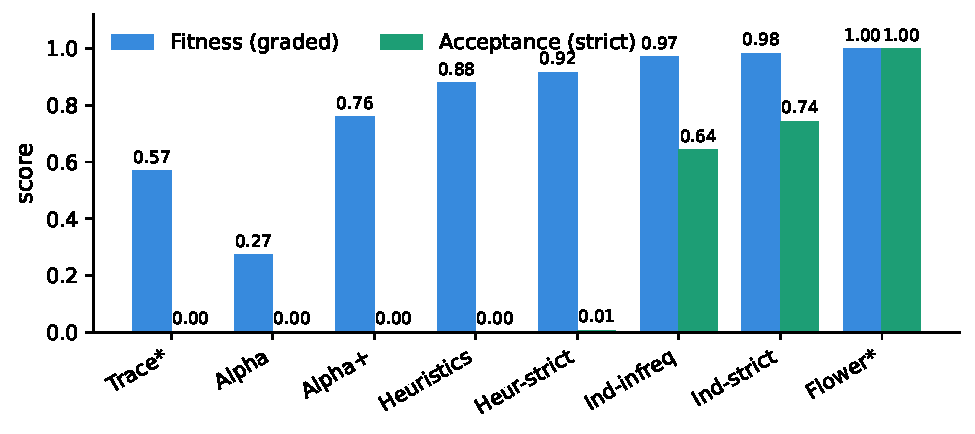
\includegraphics[width=0.92\textwidth]{figures/fig_accept_d1.pdf}
\caption{Two readings of the shadow log on D1 Sepsis: graded fitness (partial credit) vs.\ strict acceptance (perfect-replay fraction). Acceptance gives the construct's clean poles (Trace $0.00$, Flower $1.00$), and the gap between the bars exposes partial-credit inflation: e.g.\ Alpha+ scores $0.76$ fitness but $0.00$ acceptance, and the trace model $0.57$ fitness but $0.00$ acceptance.}
\label{fig:accept}
\end{figure}

\begin{table}[t]
\centering
\caption{Acceptance reading on D1 (\genaccept) vs the acceptance ground truth (R1-accept).}
\label{tab:accept}
\setlength{\tabcolsep}{3.5pt}
\footnotesize
\begin{tabular}{@{}lcccccccc@{}}
\toprule
 & Trace & Alpha & Alpha$+$ & Heur. & Heur.S & Ind.Inf & Ind.S & Flower \\
\midrule
\genaccept{} & .000 & .000 & .000 & .001 & .008 & .644 & .744 & 1.00 \\
R1-accept & .000 & .000 & .000 & .028 & .043 & .783 & .996 & 1.00 \\
\bottomrule
\end{tabular}
\end{table}

Three observations. The poles anchor on \chg{every dataset}, in both metric and ground truth: the flower model at $1.000$ exactly, the trace model at or below $0.003$\chg{; the largest deviation (D5's $0.003$) is the \texttt{duplicates\_kept} integrity counter surfacing, the dedup retry cap keeping $2$ to $3$ observed variants per $1{,}000$ on the most repetitive log}. These are the clean $0/1$ bounds that graded fitness cannot provide. Near-zero acceptances are true model properties, not metric failures: on D1 the ground truth itself shows Alpha, Alpha+, and both Heuristics models strictly accepting (almost) no unseen real traces (e.g., Alpha+ $0.000$, Heuristics $0.028$); only the Inductive family genuinely accepts novel behavior. Alpha+'s graded $0.83$ under R1 is thus pure partial credit, and the per-model gap between \genshadow{} and \genaccept{} is itself diagnostic. Caveats: strict acceptance is bimodal and sensitive to net soundness (which is why it accompanies rather than replaces the graded score), rank correlation is uninformative under mass ties at zero (use Pearson/MAE), and \genaccept{} underestimates R1-accept in the mid-range on D1 because shadow traces (containing novel recombinations and mutations) are deliberately harder than held-out real traces.

\chg{D4 exposes a depth limit of the strict reading, and we report it as a finding rather than smoothing it away. On D4 (mean trace length $57.4$) even held-out real traces barely replay perfectly: the ground truth's largest value is $0.30$ (Inductive-strict), and our shadow traces, which deliberately contain novelty, almost never do ($0.0002$ on that cell). Every other D4 cell is near zero on both axes, so only two mid-range cells carry signal, Pearson is uninformative on D4, and MAE stays at $0.057$. The cause is mechanical: one deviation anywhere in a 57-event trace breaks a perfect replay, so strict acceptance saturates toward $0$ as traces deepen. The poles still anchor exactly. This is a property of membership-shaped generalization at depth, not of our generator, and it is one more reason the graded score is the headline and acceptance the diagnostic.}

\chg{We also quantified the proxy error flagged in Sect.~\ref{sec:impl:deviations}: on D1 shadow traces ($1{,}000$ per net), the token-replay flag agrees with cost-zero alignments exactly ($1.0000$) on the Inductive-strict, Flower, and Heuristics nets, and reaches $0.804$ on Inductive-infrequent, where all $196$ disagreements are one-directional over-accepts of the replay flag (invisible-transition leniency). Mid-range acceptance values on that net class are therefore upper bounds; the poles and the validation above are unaffected.}

{\color{chgblue}
\subsection{The generator premise, tested directly}
\label{sec:eval:genval}
The central premise of the metric is that the shadow log resembles valid future behavior. The earlier draft argued this constructively; the claim is now measured. For every R1 fold partition ($3$ shuffles $\times$ $5$ folds per log), we train the generator on the train fold only, generate $1{,}000$ traces, and count how many are exact activity-sequence matches of variants in the held-out test fold. The generator deduplicates against its own training variants, and train and test folds share no variants, so a hit cannot be memorization: it is a real future variant the generator produced without ever seeing it. Two baselines calibrate the number: the 1-gram ablation, and uniformly random traces over the training alphabet and length distribution.

\begin{table}[t]
\centering
\caption{Generator premise: share of generated traces that exactly match held-out real variants (mean over $15$ folds, in \%), and the share of the held-out variant set reached (coverage, in \%). TLRA (trace-based log representativeness, Table~\ref{tab:datasets}) is repeated here: the hit-rate tracks it at Pearson $0.97$.}
\label{tab:genval}
\setlength{\tabcolsep}{5pt}
\footnotesize
\begin{tabular}{@{}lrrrrr@{}}
\toprule
Log & TLRA & ShadowGen & 1-gram & Random & Coverage \\
\midrule
D1 & 0.19 & 1.1 & 0.4 & 0.0 & 4.8 \\
D2 & 0.80 & 16.6 & 10.9 & 0.01 & 10.6 \\
D3 & 0.49 & 8.6 & 0.0 & 0.0 & 1.4 \\
D4 & 0.35 & 0.09 & 0.0 & 0.0 & 0.01 \\
D5 & 0.95 & 25.9 & 5.5 & 0.0 & 1.7 \\
\bottomrule
\end{tabular}
\end{table}

Four readings of Table~\ref{tab:genval}. First, the premise holds: on D5 a quarter of the generated traces are unseen real future variants, and random traces are essentially never one (the only nonzero random cell is $0.01\%$ on D2's four-activity alphabet). Second, deep context is what produces the realism where it matters: on D3 the full model hits $8.6\%$ of the time and the 1-gram ablation never does. Third, the exact-match criterion is length-limited by construction: a hit must reproduce every step, so the rate falls steeply with trace depth. D4 at $57$ events per trace is near zero for that reason alone; its graded calibration (MAE $0.016$) shows the generator models D4 well, and the drop mirrors the strict-acceptance saturation of Sect.~\ref{sec:eval:accept}. A fold sweep confirms depth rather than undertraining as the cause: under $k\in\{2,5,10\}$ the hit-rate scales with the size of the held-out pool as expected, and D4 stays near zero on every split ($\le 0.17\%$), even when trained on $90\%$ of its variants. Exact matches are therefore a conservative lower bound on the shadow log's realism, and even this bound is orders of magnitude above chance. Fourth, the exact-match rate is a structural property of the log, not a measure of generator quality: it tracks representativeness at Pearson $0.97$ with TLRA (D4 the depth exception). This inverts the calibration result of Sect.~\ref{sec:eval:scale}, where TLRA was refuted as a predictor: representativeness governs how often future behavior can be exact-matched, but not how well the metric calibrates. The generator produces real future behavior regardless of representativeness; it is merely easier to exact-match on repetitive logs, in line with the observation that a highly representative log can stand in for the system directly~\cite{karunaratne2024representativeness}.

Exact match is a floor. By Levenshtein distance on activity sequences, the shadow log stays close to real behavior even where exact reproduction is out of reach: the share of generated traces within three edits of a held-out variant is $44\%$ on D1, $91\%$ on D2, $47\%$ on D3, $2\%$ on D4, and $80\%$ on D5, against at most $4.6\%$ for random. The deep-context gap widens under this measure: on D3 the full model reaches $47\%$ while the 1-gram reaches $0.3\%$; on the short repetitive D5 the 1-gram instead edges ahead ($90\%$ against $80\%$). D4 stays low because three edits on a $57$-event trace is about a $5\%$ tolerance, but both the 1-gram and random floors are zero there, so the $2\%$ is real signal.

Beyond the five primary logs, the premise holds across the full 21-log catalog (Fig.~\ref{fig:genvalbox}): the shadow log's exact-match rate meets or exceeds the random floor on every log, strictly on $19$ of $21$ (the two ties are the deepest logs, where both are zero), and random never exceeds $2.2\%$. Exact-match magnitude tracks log size and trace depth, so the five primary logs carry the detail.
}

\begin{figure}[t]
\centering
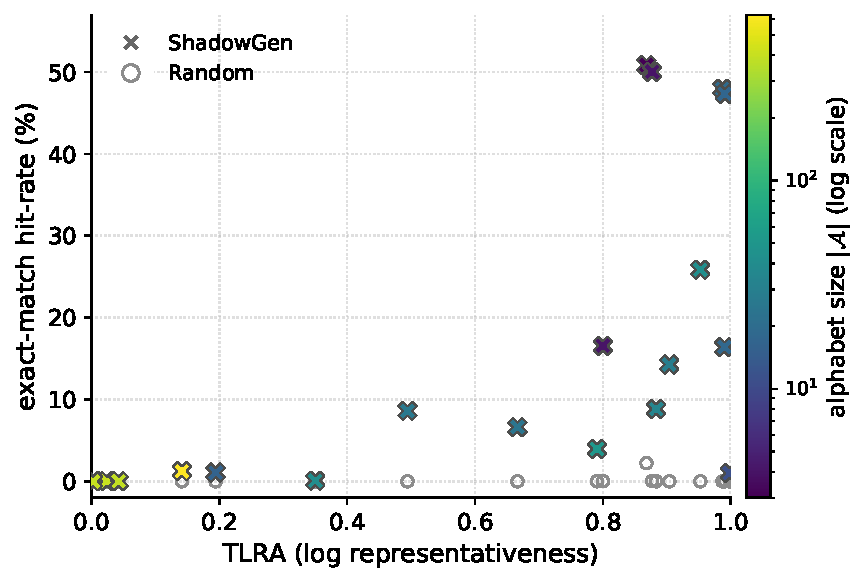
\includegraphics[width=0.55\textwidth]{figures/fig_genval_box.pdf}
\caption{Generator premise across the 21-log catalog: exact-match rate of the shadow log vs uniformly random traces, one point per log. Random is pinned near zero (its lone $2.2\%$ point is a $108$-variant log); the shadow log exceeds it on $19$ of $21$ and ties at zero on the two deepest.}
\label{fig:genvalbox}
\end{figure}

\subsection{Runtime}
\label{sec:eval:runtime}
\chg{The metric evaluates one cell ($5\times1{,}000$ traces) in a median of $3$ seconds on the two small logs (maximum $18$) and at a median of $14.9$ seconds per model over all five logs; the worst cell is $22$ minutes (D4, Inductive-strict, where replay on the discovered net dominates). The bootstrap adaptation has the same shape at $2.5\times$ the cost (median $36.9$\,s). The references are of a different order: R1 has a median of $19$ minutes per model on D4 and a worst cell of $5.7$ hours, and leave-one-variant-out reaches $46$ hours on a single cell. AVATAR exceeds the budget on every log (Sect.~\ref{sec:eval:feasibility}). Figure~\ref{fig:pareto} sets accuracy against time over the whole benchmark.} Among methods that agree with the ground truth, ours is the fastest, and it stays defined where the ground truth is not: it scores a model artifact in hand, without rediscovery (Sect.~\ref{sec:method:complexity}).

\begin{figure}[t]
\centering
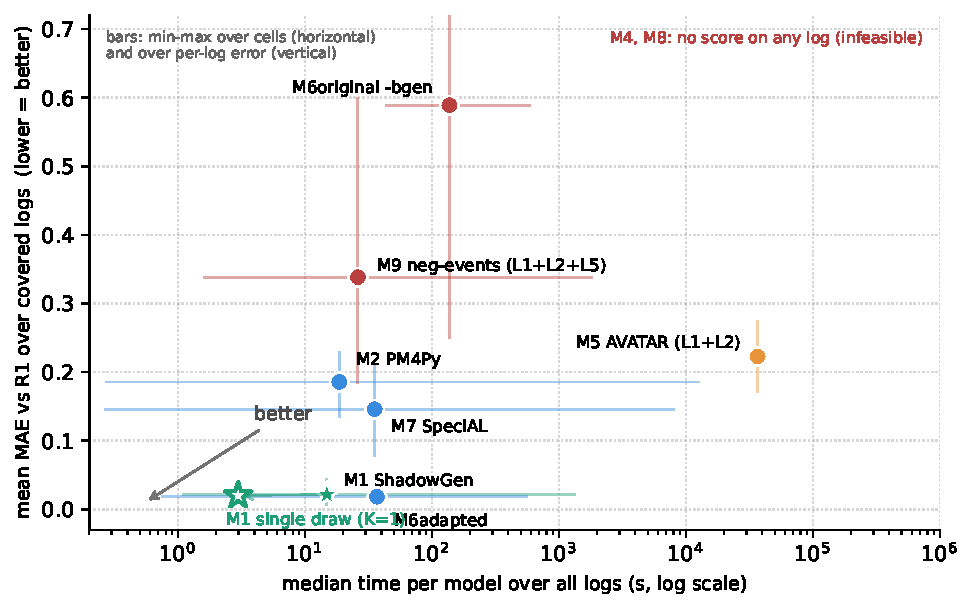
\includegraphics[width=0.85\textwidth]{figures/fig_pareto_scale.pdf}
\caption{\chg{Speed against accuracy over all five logs: median time per model (log scale) versus mean of the per-log MAEs to R1; lower-left is better. Whiskers show the spread the aggregates hide: horizontal, min to max cell runtime; vertical, min to max per-log MAE. ShadowGen and the bootstrap adaptation are alone in the accurate corner; PM4Py is fast but never accurate; the Entropia \texttt{-bgen} F-measure is slow and far off; AVATAR is a budget sentinel on all five logs, plotted at its projected CPU cost (${\sim}3$--$4$ days per log, from a measured anchor; Sect.~\ref{sec:eval:feasibility}) without a time whisker; its accuracy is read from the two small logs it scores off-protocol. M4 and M8 do not complete a scorable comparison.}}
\label{fig:pareto}
\end{figure}

\subsection{Discussion}
\label{sec:eval:discussion}
\chg{On five real-life logs spanning $15$ thousand to $2.5$ million events,} the methods that confront a model with resampled or synthesized behavior (our metric, bootstrap) agree with the cross-validation ground truth in both rank and absolute value, whereas methods that inspect structure or aggregate diversity (PM4Py, SpeciAL) do not\chg{, on any log}. This supports the project's core hypothesis: generalization is a claim about unseen behavior and is therefore best measured by probing models with plausible unseen behavior, instead of analysing the existing structure. \chg{That two independently designed generators land on the same calibration strengthens the point: the paradigm carries the result, and our generator adds interpretability, principled novelty, and a $2.5\times$ speed advantage on top of it.} Our metric reaches this agreement at interactive runtime with interpretable internals (per-context novelty, mutation flags, the openness profile, the acceptance reading) that neural and bootstrap aggregates do not expose. The honest claim is therefore not ``best metric'' but ``matches the strongest baseline's calibration while probing genuinely unseen behavior that resampling cannot reach, and exposing why a model scored as it did, at comparable cost and with no external toolchain.''

\subsection{Threats to validity}
\label{sec:eval:threats}
\chg{Breadth: the study covers five logs and eight miners per log, but every correlation is computed over six non-degenerate miners (four for SpeciAL on D5 and three for the Entropia \texttt{-bgen} tool on D4, as flagged), a deliberately small, interpretable sample (a D1 check over eleven configurations gives the same calibration, Sect.~\ref{sec:eval:external}); dataset-specific structure can still favor particular methods, and the AVATAR comparison rests on two off-protocol small-log scorecards read for the construct litmus, so its verdict is correspondingly limited.}

Shared measurement core: the metric, R1, R3, and M6adapted all score via token replay, so part of their mutual agreement may reflect a shared fitness notion rather than shared generalization semantics. R1's per-fold rediscovery limits but does not eliminate this, and the acceptance reading was already validated against a separately computed ground truth (R1-accept). \chg{We also tested the shared engine directly: recomputing R1 on D1 with cost-zero alignments, a conformance engine independent of token replay, leaves ShadowGen's ranking unchanged (Spearman $1.0$, Pearson $0.96$ over the five sound nets), so the agreement is not an artifact of the shared engine. Alignment fitness is moreover undefined on unsound nets, since the alignment tool refuses Alpha+, which token replay scores; that is one reason the metric uses token replay.}

Ground truth and representativeness: our validation rests on agreement with variant-based hold-out (R1/R2), the strongest available empirical reference because its test traces are provably valid where a shadow trace is only plausible by construction. Both are computed from the log, so both are only as faithful to the system as the log is representative of it, a responsibility of the data-gathering stage rather than of the metric (Sect.~\ref{sec:related}). \chg{The registered prediction that our calibration error grows as representativeness falls was tested and refuted (Sect.~\ref{sec:eval:scale}); the bound is real, but TLRA alone does not govern it.}

\chg{Generator validity: the premise that the shadow log resembles valid future behavior is now tested directly (Sect.~\ref{sec:eval:genval}): up to $25.9\%$ of generated traces are exact held-out real variants, against at most $0.01\%$ for random traces. The residual threat is that exact matching is a lower-bound criterion: on deep-trace logs it cannot certify realism (D4: $0.09\%$), where the premise is supported only indirectly by the graded calibration and by the near-match reading ($2\%$ of D4 traces within three edits of a held-out variant, both floors zero).}

Adapted and incomplete baselines: M6adapted uses token-replay fitness in place of the Entropia precision/recall F-measure\chg{, and its sampler is our reimplementation from the paper, validated on D1} (Sect.~\ref{sec:impl:baselines}); M3 uses a DFG approximation \chg{at scale and a proper reachability SDFA where reachability stays finite ($24$ of $40$ cells across the five logs)} (Sect.~\ref{sec:impl:baselines}); M5 has two of $3$--$5$ planned sampling runs \chg{on its off-protocol D1/D2 scorecards, and its budget sentinels on all five logs are evidence-based (Sect.~\ref{sec:eval:feasibility})}; \chg{M7's D5 cells use a newer package version than D1--D4 (Sect.~\ref{sec:impl:baselines})}; R2 sampled $50$ of $846$ variants on D1\chg{, and the D4 Inductive-strict cell of R2 is sampled at $50$ of $28{,}457$ variants (a full leave-one-variant-out there would need $28{,}457$ rediscoveries)}.

Calibration provenance: $N{=}6$ was selected on one log via a proxy criterion (mutation rate), and the mutated-trace share varies strongly across logs ($\sim4\%$ on BPI 2017 vs.\ $\sim50\%$ on Sepsis), so proposal-distribution effects are dataset-dependent by construction. \chg{Relatedly, the variable-order model's advantage over its 1-gram floor is itself log-dependent: on short, simple logs the 1-gram can match or exceed it (Sect.~\ref{sec:eval:scale}); deep context pays off specifically where decisions depend on it.} \chg{A sweep over $N$ and $\tau$ confirms the setting is not fragile: calibration MAE is a broad plateau for $N\ge4$ (D1 $0.020$ to $0.029$, D3 $0.005$ to $0.007$; $N{=}6$ within noise of the optimum) and barely moves with $\tau$ (at most $0.007$ across $\tau\in\{2,5,10\}$). $N{=}6$ is beaten only on the short repetitive D5, where a directly-follows generator already suffices.}

\chg{Replay reproducibility, measured: PM4Py's token replay breaks ties by element iteration order on nets with duplicate labels or silent transitions, and no seed pins it. We measured the drift across independent processes: the trace model moves by up to $0.024$, Alpha+ by up to $0.006$ (on D4), and every other cell reproduces exactly. The four-criteria agreement is essentially unaffected (the worst-case D4 MAE moves from $0.015$ to the tabulated $0.016$), and all discovery-side nondeterminism is pinned (fixed hash seed, models discovered once and cached). The acceptance proxy itself is quantified in Sect.~\ref{sec:eval:accept}.}

% =====================================================================
\section{Conclusion}
\label{sec:conclusion}

\subsubsection{Contribution and findings.}
We presented ShadowGen, a generative N-gram metric for process-model generalization, together with a strict construct definition it implements and a benchmark that validates generalization metrics against variant-based cross-validation under a four-criterion protocol with both construct poles included. \chg{The central result is that ShadowGen tracks the empirical ground truth on all five real-life logs, from $15$ thousand to $2.5$ million events: it reproduces the cross-validation ranking (at most one adjacent swap per log) and is calibrated to it (Pearson $0.986$--$0.999$, MAE $0.006$--$0.043$) at a median of $15$ seconds per model, and it does so while scoring a model in hand, where the cross-validation reference cannot. The benchmark adds findings of independent value: PM4Py is anti-correlated with empirical generalization on four of five logs and fails the flower litmus on all five; two published metrics return on too few models to be scored, and the GAN-based AVATAR exceeds the one-hour budget on all five logs; rank correlation alone is too weak a validation criterion; an independently designed bootstrap generator lands on the same calibration, corroborating the generative paradigm; the acceptance reading anchors the construct poles and exposes partial-credit inflation; and the generator premise is confirmed directly across the 21-log catalog (up to $25.9\%$ of generated traces are exact held-out variants).}

\subsubsection{Limitations.}
The metric and much of its cross-validation reference share a token-replay core, so part of their agreement reflects a shared conformance notion rather than shared generalization semantics (an alignment-based recomputation of R1 keeps the ranking, so the residual concern is calibration-level, Sect.~\ref{sec:eval:threats}); the context order $N{=}6$ is calibrated on a single log via a proxy; several baselines are adapted, degraded, or incomplete\chg{; the strict acceptance reading saturates on deep-trace logs and its membership test is a replay proxy with a measured one-sided error on one net class ($0.804$ agreement on Inductive-infrequent)}.

\subsubsection{Future work.}
\chg{The natural next steps are an alignment-based acceptance reading that removes the replay proxy and an AVATAR comparison under a GPU budget, so the second generative paradigm can be judged at scale. A proper stochastic-automaton conversion of entropic relevance is not among them: we implemented it (Sect.~\ref{sec:eval:feasibility}), and it fails the flower litmus.} The metric itself is feature-frozen, with the \texttt{mle} mode as the default and the name ShadowGen reflecting its purely generative design.

% =====================================================================
% DECLARATION ON THE USE OF AI-BASED TOOLS
% No Informatics-specific template found; using a one-line declaration.
% Revisit if the chair requires a specific format or a per-author tool list.
% =====================================================================
\section*{Declaration on the Use of AI-Based Tools}
In preparing this work, we used AI-based assistants (large-language-model and coding
tools) for source-code drafting, figure generation, and language editing; all content
was reviewed and verified by the authors, who take full responsibility for it.

% =====================================================================
\appendix
\section{Per-log acceptance agreement}
\label{sec:appendix:accept}
\chg{Table~\ref{tab:accept-scale} reports the acceptance reading's agreement with the acceptance ground truth (R1-accept) on every log, the per-log companion to the graded-fitness scale table (Table~\ref{tab:scale}).}

\begin{table}[h]
\centering
\caption{Acceptance reading (\genaccept) vs the acceptance ground truth (R1-accept): agreement over the six real miners per log, plus the two construct poles. Both anchor the trace and flower poles at $0$ and $1$ on every log (largest deviation $0.003$, the D5 trace model; Sect.~\ref{sec:eval:accept}). $^{*}$Pearson is uninformative on D4: strict acceptance saturates at trace depth (mean $57$ events), leaving only two mid-range cells with signal (Sect.~\ref{sec:eval:accept}).}
\label{tab:accept-scale}
\setlength{\tabcolsep}{6pt}
\footnotesize
\begin{tabular}{@{}lrrc@{}}
\toprule
Log & Pearson & MAE & Poles (Trace\,/\,Flower) \\
\midrule
D1 Sepsis   & 0.998 & 0.076 & 0.00\,/\,1.00 \\
D2 BPI 2013 & 0.997 & 0.021 & 0.00\,/\,1.00 \\
D3 BPI 2017 & 0.992 & 0.039 & 0.00\,/\,1.00 \\
D4 BPI 2018 & \emph{n/a}$^{*}$ & 0.057 & 0.00\,/\,1.00 \\
D5 BPI 2019 & 0.999 & 0.075 & 0.00\,/\,1.00 \\
\bottomrule
\end{tabular}
\end{table}

\section{Raw cross-paradigm scores on D1}
\label{sec:appendix:external}
\chg{Table~\ref{tab:external} gives the full per-cell scores behind the D1 calibration (Sect.~\ref{sec:eval:external}): the metrics of the D1 comparison and the cross-validation references on each of the seven miners. It is the numeric backing for Figure~\ref{fig:calibration} and Table~\ref{tab:corr}; the R3-Random row is the construct floor made concrete, collapsing in the mid-permissiveness cells ($.502$, $.621$) where the real ground truth ($.902$, $.933$) does not.}

\begin{table}[h]
\centering
\caption{D1 Sepsis: scores per miner, mean $\pm$ std where applicable (seven miners of the external comparison). $^{\ddagger}$model fitness $<0.5$ on the log. $^{\dagger}$returns too few comparable cells (Sect.~\ref{sec:eval:feasibility}). \chg{\textsuperscript{\S}off-protocol budget sentinel (Sect.~\ref{sec:eval:feasibility}): shown for the litmus and Fig.~\ref{fig:calibration}, excluded from the agreement statistics.}}
\label{tab:external}
\setlength{\tabcolsep}{1.6pt}
\scriptsize
\begin{tabular}{@{}lccccccc@{}}
\toprule
Method & Alpha$^{\ddagger}$ & Alpha$+$ & Heur. & Heur.S & Ind.Inf & Ind.S & Flower \\
\midrule
\chg{ShadowGen (ours)} & .272$\pm$.004 & .759$\pm$.005 & .879$\pm$.002 & .917$\pm$.002 & .972$\pm$.002 & .984$\pm$.002 & 1.00 \\
M2 PM4Py & .913 & .919 & .830 & .900 & .880 & .902 & .913 \\
M5 AVATAR\chg{\textsuperscript{\S}} & .340$\pm$.020 & .562$\pm$.008 & .746$\pm$.001 & .704$\pm$.002 & .751$\pm$.002 & .535$\pm$.009 & .397$\pm$.007 \\
M6adapted$^{*}$ & .250$\pm$.010 & .775$\pm$.018 & .891$\pm$.003 & .930$\pm$.003 & .976$\pm$.003 & .994$\pm$.001 & 1.00 \\
M7 SpeciAL & .799 & .750 & 1.00 & .998 & .750 & .744 & .803 \\
M4 Anti-align.$^{\dagger}$ & \multicolumn{7}{c}{\emph{two of seven D1 cells, anti-alignment scale, not comparable}} \\
M8 Pattern$^{\dagger}$ & \multicolumn{7}{c}{\emph{no D1 cell within the hour}} \\
\midrule
R1 5-fold CV & .275$\pm$.001 & .829$\pm$.002 & .902$\pm$.005 & .933$\pm$.001 & .985$\pm$.002 & 1.00 & 1.00 \\
R2 LOVO & .306$\pm$.075 & .775$\pm$.177 & .870$\pm$.051 & .917$\pm$.044 & .981$\pm$.053 & 1.00 & 1.00 \\
R3 Random & .278$\pm$.004 & .382$\pm$.004 & .502$\pm$.005 & .621$\pm$.003 & .693$\pm$.001 & .767$\pm$.002 & 1.00 \\
\bottomrule
\end{tabular}\\[2pt]
{\scriptsize $^{*}$M6adapted scores the genuine \texttt{bsgen} bootstrap sample by token-replay fitness (a graded model--system recall, the construct the bootstrap paper defines~\cite{polyvyanyy2022bootstrap}), not the Entropia \texttt{-bgen} precision/recall F-measure (Sect.~\ref{sec:impl:baselines}). $^{\dagger}$M4 returns two D1 cells (Alpha, Heuristics-strict) as anti-alignment scores, not on this table's fitness scale, and exceeds the hour or aborts on the rest; M8 returns no D1 cell within the hour.}
\end{table}

\bibliographystyle{splncs04}
\bibliography{references}

\end{document}
